%%%%%%%%%%%%%%%%%%%%%%%%%%%%%%%%%%%%%%%%%%%%%%%%%%%%%%%%%%%%%%%%%%%%%%%%%%%%%%%%
%2345678901234567890123456789012345678901234567890123456789012345678901234567890
%        1         2         3         4         5         6         7         8
% THESIS INTRODUCTION

\chapter{Introduction}
\label{chap:introduction}
\ifpdf
    \graphicspath{{Introduction/Figures/PNG/}{Introduction/Figures/PDF/}{Introduction/Figures/}}
\else
    \graphicspath{{Introduction/Figures/EPS/}{Introduction/Figures/}}
\fi

% quote

%\setlength{\epigraphwidth}{.35\textwidth}
%\epigraph{Research is formalized curiosity.}{ Zora Neale Hurston, 1942}

% examples of sections

\section{Motivations}
\label{motivations}
A \textit{dynamic} network is a network that changes over time. This could be changes in the network topology - that is, the existence of edges and existence of nodes \cite{itdn}, or it could be changes in any attributes associated with edges and nodes such as labels or weights. Dynamic networks can be found everywhere: a road network which undergoes periodic maintenance to sections or junctions; the neural networks that form the brain where neuron activity varies; or a social proximity network where edges are created while people are close to each other and lost when they move apart. An example of a dynamic network is given in Figure \ref{exampleDynamicNetwork}.

\begin{figure}[H]
\begin{center}
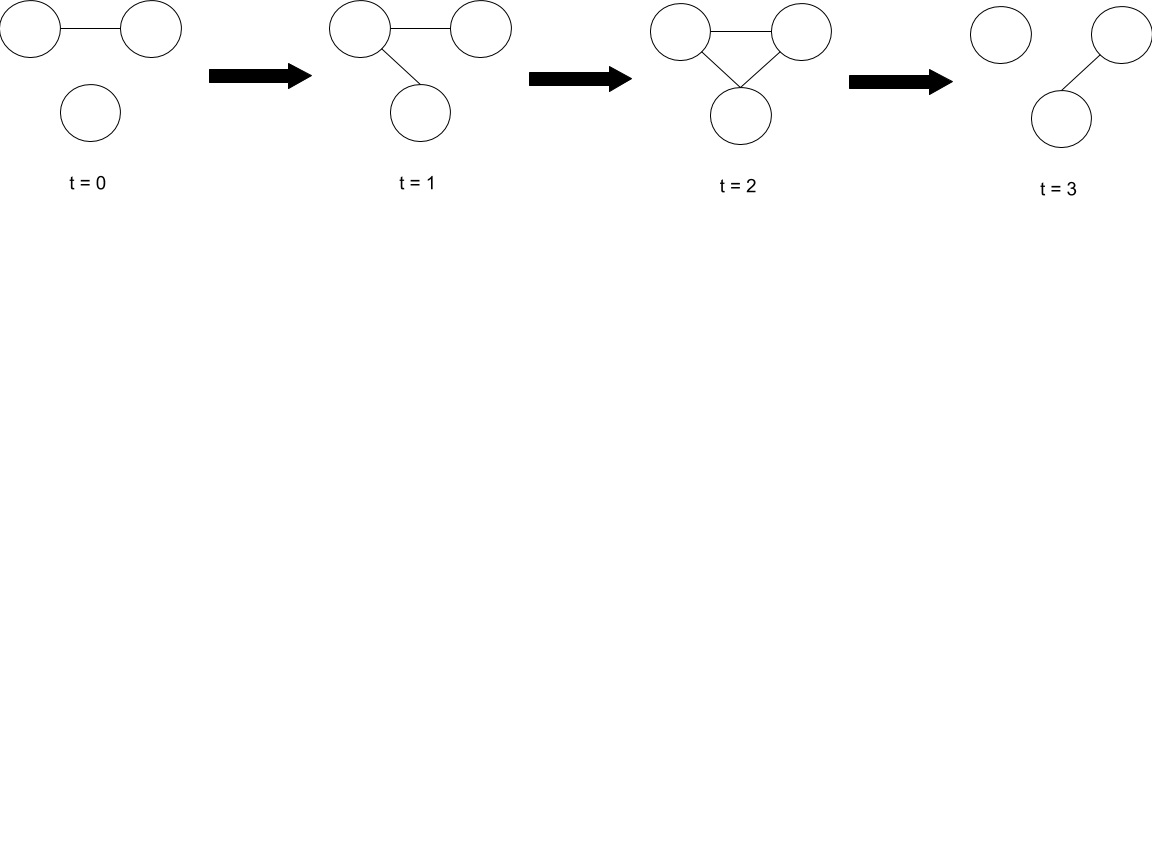
\includegraphics[trim={0 19cm 0 0}, clip, width=140mm]{./Figures/exampleDynamicNetwork.png}
\caption{An example of a dynamic network. The connections vary with time: a new connection is formed at t=1, another new connection is formed at t=2 and two are lost at t=3.}
\label{exampleDynamicNetwork}
\end{center}
\end{figure}

Naturally, dynamic networks are difficult to interpret and visualise quickly \cite{iddps}. Consider even a simple network composed of a handful of nodes and a handful of edges. Suppose we add the dynamic element to this simple network and mutate, say, the edges through a given time period. It can be difficult to interpret what, if anything those mutations indicate or represent even on a simple network. Many different approaches have been made to try and tackle this problem and mitigate the additional cognitive load. 

This report will focus on a novel approach - using a variety of easily interpretable \textit{measures} to produce some result based on either an aspect of the network at each frame of time or on the graph overall, for example: the density of the graph. Instead of manually stepping through the graph and attempting to pattern match, the measures can be observed. Using the measures to characterise the graph is somewhat conceptually similar to feature projection for dimensionality reduction \cite{wikidimred} in that the measures represent some feature vectors of the network and provide an abstract overview of the changes the network goes through, but since the measure visualisation is complementary to the existing network - rather than replacing it - the features aren't reduced but rather extracted and highlighted.
As more and more measures are added the resulting complexity requires that an intelligent visualisation of the measure values be implemented, since the goal is not to further add to the cognitive load but reduce it. Visualising these measures can allow us to spot patterns and trends over time, locate points of interest and motivate a hypothesis. Traditionally, network visualisations have been focused on visualising the changes themselves \cite{tsotaivg}, however here the measure-based approach aims to be more complementary to the network.

Although any type of network could have been used - care was taken while designing the measures and visualisations to keep them agnostic of the domain and avoid overfitting - a fairly small and simple social network was primarily used during development \ref{MARIEBOUCHER SOMEWHERE??}. 
%Social networks require less expert domain knowledge compared with say, biological networks to understand at a basic level [source or remove]. For the sake of simplicity I chose an easy to understand and rather small network. 
%Social networks are also more abstract than physical networks like power grids or computer networks \cite{taasodnv}.
Since this project aims to investigate dynamic network interpretation, using a simple network as a baseline ensures that difficulties in comprehension are not just inherent to the domain but to the network itself. 
%There are also a variety of existing networks that could be used to test against [source/example].
%Social network analysis provides a novel window by allowing the impacts to be quantified at the individual level, and the links between past, current and future behaviour to be carried across contexts. <https://besjournals.onlinelibrary.wiley.com/doi/pdf/10.1111/1365-2656.12764>

Networks can be constructed and interpreted in different ways. The measures used in this report are designed for a network composed of eternal nodes, unweighted edges and undirected edges, where an edge is a connection that happens instantaneously between two nodes, as in type (a) of Figure \ref{fig:edgeTypes}, and a nodepair exists between two nodes in a given period of time if any edge occurs between them in that period. 

\begin{center}
\begin{tabular}{cc}
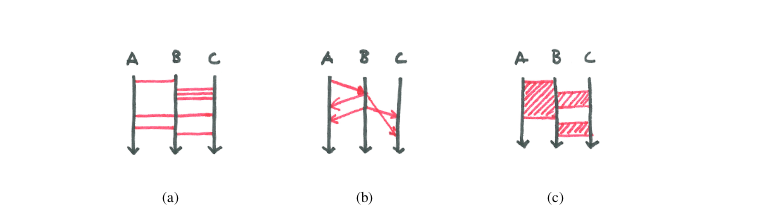
\includegraphics[trim={0 0 0 0}, width=140mm]{./Figures/edgeTypes.png}
\end{tabular}
\captionof{figure}{Types of connectivity. A, B and C represent nodes, time goes from top to
bottom, edges are indicated in red. (a) Instantaneous edges, (b) Transmissive edges, (c)
Persistent edges. \newline Figure and description taken from Connections, Changes and Cubes: Unfolding Dynamic Networks for Visual Exploration \cite{cccudnfve}.
}
\label{fig:edgeTypes}
\end{center}

Adjusting any of these assumptions would affect the selection of measures. Further work could be done on measures that take into account edge weight, persistent edges etc. The measures were also designed with social networks primarily in mind, but could of course be applied in other domains.

I extend the functionality of The Vistorian \cite{bach:hal-01205822} - an ongoing open source project by Bach et al. to create an online platform which provides interactive visualization for various kinds of networks, designed for social scientists and historians. 



%%Benjamin mentioned Objectives/Tasks section

\section{Contributions}
\label{objectives}
\begin{itemize}
    \item Summary of the literature regarding dynamic network visualisation.
    \item Development and evaluation of novel local dynamic measures - Local volatility, local activity and local redundancy.
    \item Development and evaluation of novel global dynamic measures - Global volatility, global activity and global redundancy.
    \item Extension of The Vistorian through:
    \begin{itemize}
        \item Creation of intuitive visualisations for local and global measures embedded into the existing interface.
        \item Implementing an extensible framework that ensures both new local and global measures can be easily visualised.
        \item Implementation of methods to calculate measures.
    \end{itemize}
    \item Demonstration of visualisations and measures in usage scenarios.

\section{Methodology}

To begin, I researched existing visualisation techniques for dynamic networks and various network measures. After selecting a few traditional measures I was able to implement basic prototype using those measures and a basic corresponding visualisation. I then iterated on both the visualisation and measures until the system was reasonably usable as a proof of concept. This provided a foundation to be able to add more experimental measures.

To obtain some external feedback on the progress I had made, an informal feedback meeting was held with with 4 active researchers on network analysis. These researchers were Dr Jim Lowe (James.Lowe@ed.ac.uk), Dr Miguel Garcia Sancho Sanchez (miguel.gsancho@ed.ac.uk), Mark Wong (Mark.Wong@glasgow.ac.uk) and Gil Viry (gil.viry@ed.ac.uk). I demonstrated usage of The Vistorian and the additions I had made for around 10 minutes, there was then around 15 minutes of discussion. In general there was a very positive reaction, which helped to validate the new additions and the following discussion inspired a new measure. The measures and visualisations were further iterated on, then more feedback was received from Pascal Cristofoli (pascal.cristofoli@ehess.fr). He experimented with the new additions and suggested two new measures be added as he often found himself calculating them manually. Implementing these two inspired a further two measures.  
\end{itemize}





